\documentclass[12pt,twoside]{article}

% *** Set page dimensions ***
\raggedbottom
\parindent=0in
%\setlength{\topmargin}{-0.5in}
%\setlength{\oddsidemargin}{0.1875in}
%\setlength{\evensidemargin}{0in}
%\setlength{\textheight}{8.5in}
%\setlength{\textwidth}{6.225in}
%\addtolength{\oddsidemargin}{-0.7in}
%\addtolength{\evensidemargin}{-1.2in}
%\setlength{\oddsidemargin}{-0.2in}
%\setlength{\evensidemargin}{-0.2in}
%\addtolength{\textwidth}{1.4in}
%\addtolength{\topmargin}{-.875in}
%\addtolength{\textheight}{2.00in}

% *** Packages ***
\usepackage{alltt}
\usepackage{tocloft}
\usepackage{graphicx}
\usepackage{lscape}
\usepackage{amssymb}
\usepackage{float}
\usepackage{amsmath}
\usepackage{gensymb}
%\usepackage{subfigure}
\usepackage{lscape}
\usepackage{epsfig}
\usepackage{enumerate}
\usepackage{multicol}
\usepackage{fancyhdr}
\usepackage{epstopdf}
\usepackage{hyperref}
\usepackage{listings}

% *** Table of contents and Sectioning *** 
\setcounter{secnumdepth}{0}
\setcounter{tocdepth}{5}

% *** Table of contents and Sectioning *** 
\newcommand{\next}{\addtocounter{enumi}{9} \item}
\newcommand{\now}[1]{\setcounter{enumi}{#1}}
\newcommand{\Z}{\mbox{\sf Z\hspace{-1.5mm}Z}}
\newcommand{\R}{\mbox{\rm I\hspace{-0.75mm}R}}
\columnsep=0.75in

% *** Shortcuts for syntax ***
\newcommand{\ds}{\displaystyle }
\newcommand{\vsc}{\vspace{4mm}}
\newcommand{\dd}[1]{\frac{d}{d{#1}} \,} 
\newcommand{\ddx}{\frac{d}{dx} \,} 
\newcommand{\ddy}{\frac{d}{dy} \,} 
\newcommand{\ddz}{\frac{d}{dz} \,} 
\newcommand{\dydx}{\frac{dy}{dx} \,} 
\newcommand{\dydt}{\frac{dy}{dt} \,} 
\newcommand{\dfdx}{\frac{df}{dx} \,} 
\newcommand{\ddt}[1]{  \frac{d{#1}}{dt} }
\newcommand{\pp}[2]{  \frac{\partial{#1}}{\partial {#2}} }
\newcommand{\zx}{\frac{\partial z}{\partial x} \,}
\newcommand{\zy}{\frac{\partial z}{\partial y} \,}
\newcommand{\limh}{\lim_{h \rightarrow 0} \;}
\newcommand{\diff}{\frac{d}{dx} \,}
\newcommand{\de}{\Delta}
\renewcommand{\thesection}{\Roman{section}}
\newcommand{\bfr}{\begin{flushright}}
\newcommand{\efr}{\end{flushright}}
\newcommand{\dx}{\frac{\partial f}{\partial x} \,}
\newcommand{\dy}{\frac{\partial f}{\partial y} \,}
\newcommand{\p}{\partial}
\newcommand{\vi}{\vec{i}}
\newcommand{\vj}{\vec{j}}
\newcommand{\vk}{\vec{k}}
\newcommand{\lan}{\left\langle}
\newcommand{\ran}{\right\rangle}
\newcommand{\reading}[1] { {\em Reading: #1}}
\renewcommand{\Pr}{ \mbox{Pr}}

% *** Commands related to textbook references
\newcommand{\problem}{{\bf Problem.} }

% *** Footnoting with symbols ***
\long\def\symbolfootnote[#1]#2{\begingroup%
\def\thefootnote{\fnsymbol{footnote}}\footnote[#1]{#2}\endgroup}

% *** Defining a boxed note ***
\floatstyle{boxed}
\newfloat{noteinbox}{htb}{loa}
\newenvironment{boxnote}{\begin{noteinbox}[H]}{\end{noteinbox}}

\newcommand{\Question}{ {\bf Question: }  }
\newcommand{\Example}[1]{ {\bf Example: } {\em #1} }
\newcommand{\ExampleCont}[1]{ {\em #1} }

% *** Define the boxed Week #/summary at the beginning/end of every chapter ***
\newcommand{\sectionbox}[1]{% 
\begin{tabular}{|p{6in}|}%
\hline%
\ \\ %
{\Large {\bf {#1}}}  \\%
\ \\%
\hline%
\end{tabular}}

% *** Shortcuts *** 
\newcommand\goals{\large {\bf {Goals:}}}
\newcommand\setfont{ }

% *** Week commands: overwritten in each notes file
\newcommand{\Week}{Null-InPreambleCommon}
\newcommand{\WeekTitle}{Null-InPreambleCommon}
\newcommand{\Course}{MNTC P04}
\newcommand{\SetNum}{1 }
\newcommand{\topic}[1]{
\newpage
\setcounter{page}{1}
\fancyhead[LE,RO]{#1 - \thepage}
}

% *** Setup Latex for the large version of the files ***
%\usepackage[landscape]{geometry}
\usepackage[letterpaper,landscape,hmargin={.8in,.8in},vmargin={1in,0.2in}]{geometry}

% Remove paragraph indents
\setlength{\parindent}{0pt}

% Spacing at the top for the header is too large by default
\setlength{\voffset}{-5ex}

% **** RENEW SCALING COMMANDS HERE ****
% *** Text in boxes ***
\renewenvironment{boxnote}{\begin{noteinbox}[H] \huge}{\end{noteinbox}} 

% *** Chapter lead in/summary boxes ***
\renewcommand{\sectionbox}[1]{% 
\begin{tabular}{|p{9.5in}|}%
\hline%
\ \\ %
{\huge {\bf {#1}}}  \\%
\ \\%
\hline%
\end{tabular}}

% *** 'Section'' commands, which are sometimes used for spacing
% From http://zoonek.free.fr/LaTeX/LaTeX_samples_section/0.html
\makeatletter
 \renewcommand\section{\@startsection {section}{1}{\z@}%
                                    {-3.5ex \@plus -1ex \@minus -.2ex}%
                                    {0.3ex \@plus.2ex}%
                                    {\setfont\bf}}

 \renewcommand\subsection{\@startsection {subsection}{1}{\z@}%
                                    {-3.5ex \@plus -1ex \@minus -.2ex}%
                                    {0.3ex \@plus.2ex}%
                                    {\setfont\bf}}

% *** 'Goals' should be larger in the overheads ***
\renewcommand\goals{\huge {\bf {Goals:}}}
\renewcommand\setfont{\huge }

\thispagestyle{empty}

\setfont 

\newcommand{\WeekTitleOne}{Derivatives - Foundations}
\newcommand{\WeekTitleTwo}{Derivatives - Linearization and Applications}
\newcommand{\WeekTitleThree}{Derivatives - Modeling}
\newcommand{\WeekTitleFour}{Integrals - Foundations}
\newcommand{\WeekTitleFive}{Integrals - Techniques}
\newcommand{\WeekTitleSix}{Integrals - Modeling}
\newcommand{\WeekTitleSeven}{Differential Equations - }
\newcommand{\WeekTitleEight}{Differential Equations - }
\newcommand{\WeekTitleNine}{Differential Equations - }
\newcommand{\WeekTitleTen}{Linear Algebra - }
\newcommand{\WeekTitleEleven}{Linear Algebra - }
\newcommand{\WeekTitleTwelve}{Linear Algebra - }



\begin{document}
\setfont
\pagestyle{fancy}
\renewcommand{\Week}{9 }
\renewcommand{\WeekTitle}{\WeekTitleNine }

\fancyhead[LE,RO]{Week \Week}  % default, usually only for first page
\fancyfoot{}
\sectionbox{Week \#\Week: \WeekTitle}


\vspace{5mm}
\goals
\begin{itemize}
\item Take problems that can be modeled by differential equations,
  both first and second order, and give solutions both by hand and
  MATLAB 
\item Examine case studies of differential equations applied to
  engineering problems and reproduce those solutions
\end{itemize}
\vspace{5mm}

%Falling body problem (maybe even the redbull stratos jump?)
%Electric Circuits
%Suspension cable bridge

\newpage

\topic{Application - Pendulum}
\subsection*{Application - Pendulum }
\begin{minipage}[t]{0.25\linewidth}
\vspace{0pt}
\begin{center}
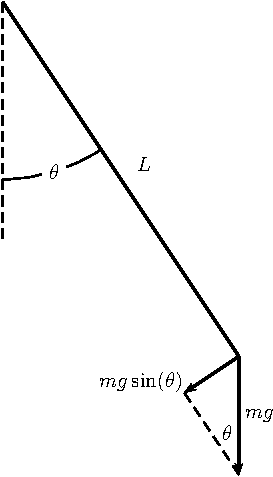
\includegraphics[width=1.0\linewidth]{graphics/notes_09_pendulum_diagram}
\end{center}
\end{minipage}
\begin{minipage}[t]{0.70\linewidth}
\vspace{0pt}
\begin{align*}
  \mbox{Newton's }& \mbox{ Second Law: } \\
   m  L^2 \theta'' & = T_g + T_f  \\
  & = - m L g \sin(\theta) - (\mu L^2 m) \theta' \\[3ex]
  \mbox{Solving for $\theta''$: }\theta'' & = - \frac{g}{L} \sin(\theta) - \mu 
  \theta'
\end{align*}
\end{minipage}

\problem Turn this single second-order DE into a pair of first-order
DEs.

\newpage


\problem Create a new MATLAB function file called \texttt{pendulumDE.m}.
Start with the first line
\begin{verbatim}
function dw_dt = pendulumDE(t, w, g, L, mu) 
\end{verbatim}

In the body of the function, implement the system of differential
equations we constructed on the previous page.
\begin{align*}
  \frac{d w_1}{dt} & = w_2 \\
  \frac{d w_2}{dt} & = -\frac{g}{L}\sin(w_1)  - \mu w_2
\end{align*}
\vsc

\newpage

\problem Write a MATLAB that simulates the motion of the pendulum
using  \\
$g = 9.8$ m/s$^2$, $L$ = 2 m, $\mu = 0.1$, and \\
initial amplitude of 0.05 radians ($\approx 2.9$ degrees).


\newpage 
\topic{Application - Period of Pendulum Swings}
\subsection*{Application - Period of Pendulum Swings}

Galileo famously noticed the consistent period of pendulum swings,
even if the amplitude of the swings was changed (so the actual
distance travelled was different).

\problem Compare the periods of the pendulum swings, using a range of
initial angles from $\theta_0 = 0.05$ radians up to $\theta_0 = 0.25$
radians ($\approx 14$ degrees).


\newpage
However, it turns out that pendulums are {\bf not} perfectly
consistent in their period, due to the non-linear term
$\ds -\frac{g}{L} \sin(\theta)$ in one of the forces: as the
amplitudes get bigger, there is a graudal lengthening of the period.


\problem Compare the periods of the pendulum swings, using a range of
initial angles from $\theta_0 = 0.25$ radians up to $\theta_0 = \frac{\pi}{2}$
radians ($= 90$ degrees).

\newpage

\topic{Pendulum -  Including an Initial Velocity}
\subsection*{Pendulum -  Including an Initial Velocity}

\problem Write a new simulation script that starts the pendulum
swinging from $ \theta_0 = -\frac{\pi}{2}$, with no initial velocity.
Simulate the motion for this scenario.

Use the  parameters $g = 9.8$ m/s$^2$, $L$ = 2 m, and $\mu = 0.1$. \\

\vsc

\newpage

\problem If we keep the initial angle at $-\frac{\pi}{2}$ (pendulum
out horizontally), experiment and find the initial velocity that will
push the pendulum ``over the top''.

\newpage

\topic{Deformation of a Loaded Beam}
\section*{Deformation of a Loaded Beam} 
~\\[1ex]

\begin{minipage}{3.2in}
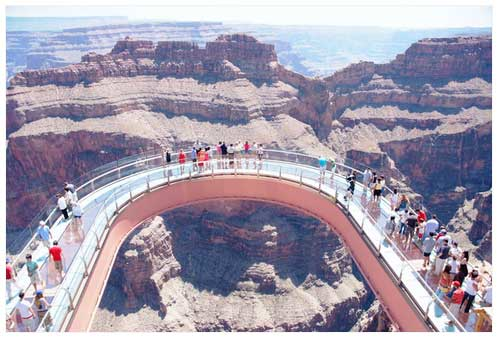
\includegraphics[width=3in]{graphics/notes_09_GrandCanyonWalkway} \\
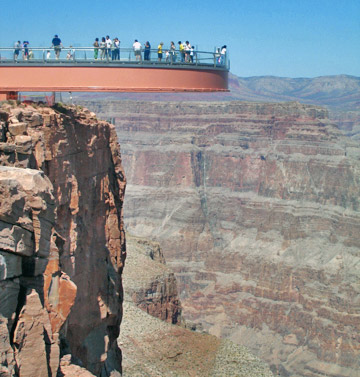
\includegraphics[width=3in]{graphics/notes_09_GrandCanyon_SkywalkFromOutsideLedge}
\end{minipage}
\begin{minipage}{4in}
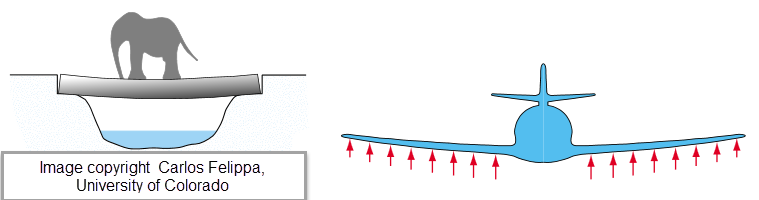
\includegraphics[width=7in]{graphics/notes_09_BeamExamples_CarlosFelippa} \\
\end{minipage}

\newpage

The shape of a beam under load is defined by the differential equation

$$EI y^{(4)} = p(x)$$
where 
\begin{itemize}
\item $y(x)$ is the deflection (distance away from a straight line),  
\item $p(x)$ is the loading in N/m at point $x$ along the beam, 
\item $E$ is the modulus of elasticity of the beam (depends on material), and  
\item $I$ is the moment of inertia of the beam (depends on beam shape and size) 
\end{itemize}

Also relevant are the properties 
\begin{align*}
  V_0 & = \mbox{shear}(0) = \int_0^L p(x)~dx \mbox{ and }\\
  M_0 & = \mbox{torque}(0) = \int_0^L x ~p(x)~dx 
\end{align*}

 \newpage


\topic{Cantilevered Beam Under Uniform Load - Method A}  
\subsection*{Cantilevered Beam Under Uniform Load} 

 Under a uniform loading (constant force per unit length), a {\em
   cantilevered beam} which is $L = 2$ m long, made out of a pine ``2 by 4'' satisfies \\
 $p(x) = 100$ N/m, (or roughly 10 kg applied to each meter) \\
 $I = 2.23 \times 10^{-6}$ m$^4$,\hspace{0.5in} $E = 9.1 \times
 10^{9}$ N/m$^2$,

 \begin{center}
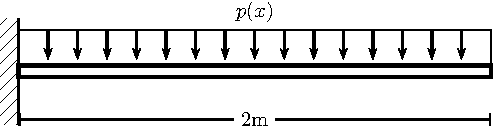
\includegraphics[width=0.6\linewidth]{graphics/notes_09_beams1}
 \end{center}

and the initial conditions \\
$y(0) = 0$, $y'(0) = 0$, $y''(0) = V_0$, and $y'''(0) = M_0$.

\newpage

\problem Find the amount of deflection of the beam at the tip under
this load, using {\bf multiple integrals}.

\begin{minipage}[t]{0.5\linewidth}
\vspace{0pt}
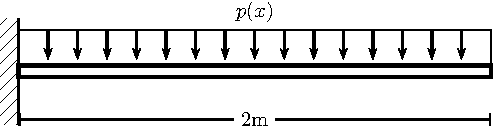
\includegraphics[width=1.0\linewidth]{graphics/notes_09_beams1}
\end{minipage}
\hfill
\begin{minipage}[t]{0.45\linewidth}
\vspace{0pt}
$EI y^{(4)} = 100$ \\
$y(0) = 0$, $y'(0) = 0$,  \\
$y''(0) = V_0$, and $y'''(0) = M_0$.
\end{minipage}

\newpage
\topic{Cantilevered Beam Under Uniform Load - Method B}  
\subsection{Cantilevered Beam Under Uniform Load - Differential Equation}  

\problem Find the amount of deflection of the beam at the tip under
this load, using a {\bf differential equation solver}.

\begin{minipage}[t]{0.5\linewidth}
\vspace{0pt}
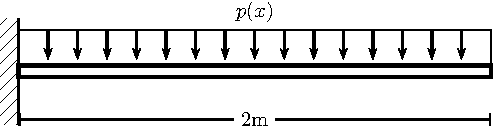
\includegraphics[width=1.0\linewidth]{graphics/notes_09_beams1}

%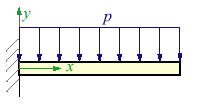
\includegraphics[width=3in]{graphics/notes_09_CantileveredBeam_Diagram}
\end{minipage}
\begin{minipage}[t]{0.5\linewidth}
\vspace{0pt}
$EI y^{(4)} = 100$ \\
$y(0) = 0$, $y'(0) = 0$,  \\
$y''(0) = V_0$, and $y'''(0) = M_0$.
\end{minipage}

\newpage
\problem If the maximum allowable deflection in such a beam is only
0.2 cm (say in a building code), what would the maximum uniform load
be?

\newpage

\topic{Cantilevered Beam - Non-Uniform Load}
\subsection*{Cantilevered Beam - Non-Uniform Load}

\begin{minipage}[t]{0.55\linewidth}
\vspace{0pt}
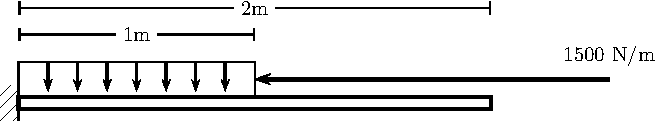
\includegraphics[width=1.0\linewidth]{graphics/notes_09_beams2}
\end{minipage}
\begin{minipage}[t]{0.45\linewidth}
  \vspace{0pt}
  $EI y^{(4)} = 100$ \\
  $y(0) = 0$, $y'(0) = 0$,  \\
  $y''(0) = V_0$, and $y'''(0) = M_0$.
\end{minipage}

\problem Use a differential equation solver to generate a plot of the
deflection of the beam shown above, for a $2\times10$ wood beam:
$I = 4.1 \times 10^{-5}$ m$^4$, and $E = 9 \times 10^9$ N/m.

\newpage

\topic{Application - Simple Lake Scenario}
\subsection{Application - Simple Lake Scenario}
\begin{problem}
  Consider a small lake that initially contains $10$ million litres of
  fresh water.  Water containing an undesirable chemical flows into
  the pond at the rate of $5$ million litres per year; the mixture in
  the pond flows out at the same rate.  The concentration $\rho(t)$ of
  chemical in the incoming water varies periodically with time
  according to the expression
  $\rho(t) = 2 + \sin(2t) \; \text{g} \cdot \text{L}^{-1}$.
  \begin{enumerate}
  \item Construct a mathematical model of this flow process.
\newpage
\item Use MATLAB and a differential equation solver to determine the
  amount of chemical in the pond at any time.

\newpage
~
\newpage
  \item Describe the effect of the variation in the incoming concentration.
  \end{enumerate}
\end{problem}

\newpage
~ 
\newpage

\topic{Application - Tailings Pond With Sediment}
\subsection*{Application - Tailings Pond With Sediment}
% Source: http://faculty.sfasu.edu/judsontw/ode/html/firstlook05.html
Consider another tailings pond, where the the inflow contains
sediments that will settle out of the water.

In this pond, the volume is 40,000 cubic meters.  
\begin{itemize}
\item Water is flowing in and out of the pond at a rate of 2,000 cubic
  meters per day.
\item The water flowing into the pond contains 2 g of toxic chemical
  per cubic meter.
\item The inflow water also contains 
\end{itemize}

\problem Sketch a diagram of this scenario.

\newpage

Write a differential equation that describes


\newpage
\topic{Application - Interconnected Tanks}
\section*{Application- Interconnected Tanks}

\noindent
Consider the tanks shown below, which shows water flowing between the
tanks, and the concentration of a salt solution coming in.  Within
each tank, the water/salt solution is kept well mixed.
\begin{center}
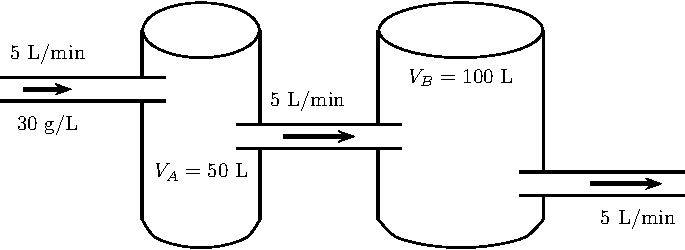
\includegraphics[width=0.7\linewidth]{graphics/notes_09_tanks1}
\end{center}

\begin{problem}
  If both tanks start with no salt, sketch what you expect will happen
  to the concentration within each tank over time.
\end{problem}

\newpage
\begin{minipage}[h]{0.5\linewidth}
\vspace{0pt}
\begin{problem}
Create a system of differential equations that dictate 
how the two tank concentrations will evolve over time.
\end{problem}
\end{minipage} \hfill
\begin{minipage}[h]{0.45\linewidth}
\vspace{0pt}
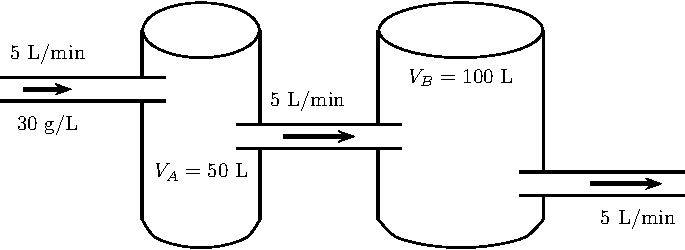
\includegraphics[width=1.0\linewidth]{graphics/notes_09_tanks1}
\end{minipage}


\newpage
\topic{Tank System - Example 1}
\begin{minipage}[h]{0.5\linewidth}
\vspace{0pt}
\begin{problem}
  Predict the exact salt concentrations over time by 
  solving the system of linear differential equations
  \begin{align*}
\frac{d}{dt}    
\begin{bmatrix} c_A \\ c_B 
    \end{bmatrix}
=
\begin{bmatrix}
  \frac{-1}{10} & 0 \\
  \frac{1}{20} &   \frac{-1}{20}   
\end{bmatrix}
\begin{bmatrix} c_A \\ c_B 
    \end{bmatrix}
+ 
\begin{bmatrix}
  3 \\ 0 
\end{bmatrix}
  \end{align*}
\end{problem}
\end{minipage} \hfill
\begin{minipage}[h]{0.45\linewidth}
\vspace{0pt}
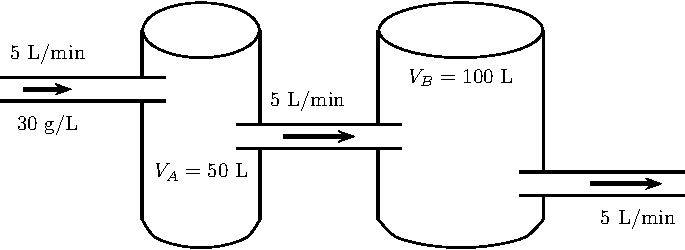
\includegraphics[width=1.0\linewidth]{graphics/notes_09_tanks1}
\end{minipage}

\newpage
\hfill 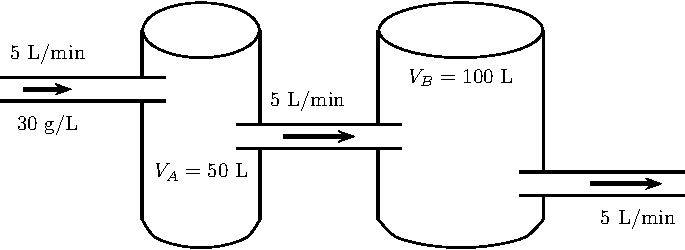
\includegraphics[width=0.5\linewidth]{graphics/notes_09_tanks1}

\newpage
\hfill 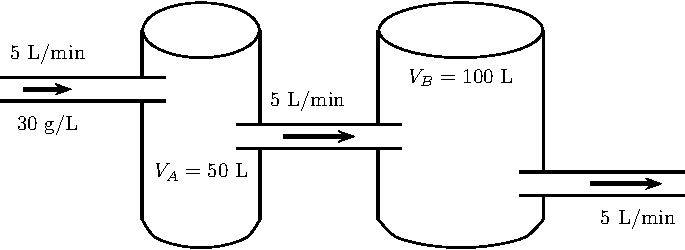
\includegraphics[width=0.5\linewidth]{graphics/notes_09_tanks1}

\newpage
\hfill 
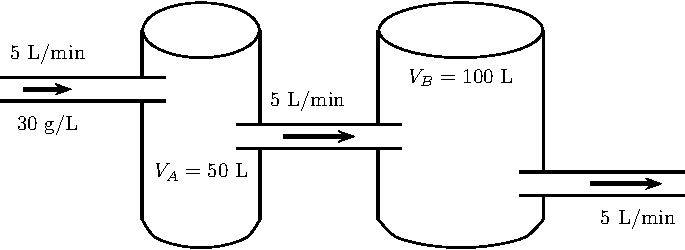
\includegraphics[width=0.3\linewidth]{graphics/notes_09_tanks1}

\begin{align*}
  c_A & = -30 e^{-t/10} + 30; \\
c_B & = 30 e^{-t/10} - 60 e^{-t/20} + 30
\end{align*}

\begin{center}
%  \includegraphics[width=0.8\linewidth]{graphics/w11_tank_graph_1}
\end{center}



% \begin{proof}[Solution]
%   Let $Q_A(t)$ and $Q_B(t)$ denote the amount (in kg) of salt in tanks $A$ and
%   $B$ respectively at time $t$ (in minutes).  It follows that
%   \begin{align*}
%     Q_A'(t) &= \text{input rate} - \text{output rate} = (5 \; \text{L} \cdot
%     \text{min}^{-1})(3 \; \text{kg} \cdot \text{L}^{-1}) - (5 \; \text{L} \cdot
%     \text{min}^{-1}) \left( \frac{Q_A \; \text{kg}}{50 \; \text{L}} \right) = 15
%     - \frac{Q_A}{10} \\
%     Q_B'(t) &= (5 \; \text{L} \cdot \text{min}^{-1}) \left( \frac{Q_A \;
%         \text{kg}}{50 \; \text{L}} \right) - (5 \; \text{L} \cdot
%     \text{min}^{-1}) \left( \frac{Q_B \; \text{kg}}{50 \; \text{L}} \right) =
%     \frac{Q_A}{10} - \frac{Q_B}{10} \, .
%   \end{align*}
%   In particular, we obtain
%   \begin{xalignat*}{7}
%     \frac{dQ_A}{dt} &= \frac{150 - Q_A}{10} &&\Longrightarrow & \int
%     \frac{dQ_A}{Q_A-150} &= \int - \frac{1}{10} \; dt &&\Longrightarrow & \ln |
%     Q_A - 150|  &= -\tfrac{1}{10}t + K \\
%     &&&\Longrightarrow & Q_A(t) &= 150 - C e^{-t/10} \, .
%   \end{xalignat*}
%   Since $Q_A(0) = 50$, we have $C = 100$ and $Q_A(t) = 150 - 100 e^{-t/10}$.
%   Hence, we have
%   \begin{align*}
%     \frac{dQ_B}{dt} + \frac{1}{10} Q_B &= 15 - 10e^{-t/10} \, ,
%   \end{align*}
%   so the integrating factor is $\exp\left( \displaystyle\int \tfrac{1}{10} \;
%     dt \right) = e^{t/10}$ which gives
%   \begin{align*}
%     \frac{d}{dt} \Bigl( e^{t/10} Q_B \Bigr) &= e^{t/10} \left( \frac{dQ_B}{dt} +
%       \frac{1}{10} Q_B \right) = e^{t/10} \Bigl( 15 - 10e^{-t/10} \Bigr) = 15
%     e^{t/10} - 10 \\
%     e^{t/10} Q_B &= \int 15 e^{t/10} - 10 \; dt = 150 e^{t/10} - 10 t + C' \\
%     Q_B(t) &= 150 - 10te^{-t/10} + C' e^{-t/10} \, . 
%   \end{align*}
%   Since $Q_B(0) = 100$, we have $C' = -50$ and $Q_B(t) = 150 - 10te^{-t/10} + C'
%   e^{-t/10}$.
% \end{proof}
\newpage

\topic{Tank Model - Example 2}

Consider the more complicated tank arrangement shown below.
\begin{center}
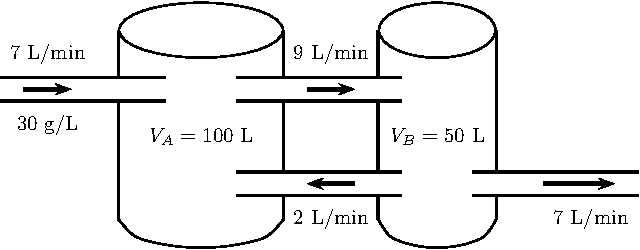
\includegraphics[width=0.7\linewidth]{graphics/notes_09_tanks2}
\end{center}
\begin{problem}
Given that the initial concentrations are \\
$c_A(0) = 0 $ g/L and $c_B(0)  = 90$ g/L,  \\
sketch what you would predict for the concentration in each tank over time.
\end{problem}

\newpage
\begin{minipage}[h]{0.5\linewidth}
\vspace{0pt}
\begin{problem}
  Construct the differential equation for the salt concentration in
  each tank, and write it in matrix form.
\end{problem}
\end{minipage} \hfill
\begin{minipage}[h]{0.45\linewidth}
\vspace{0pt}
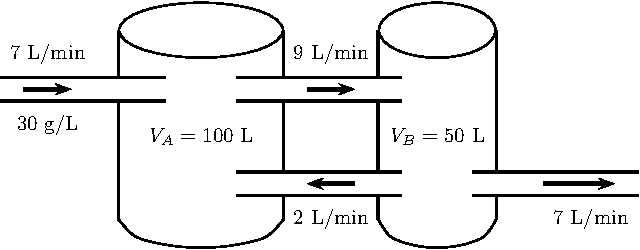
\includegraphics[width=1.0\linewidth]{graphics/notes_09_tanks2}
\end{minipage}

\newpage
\hfill 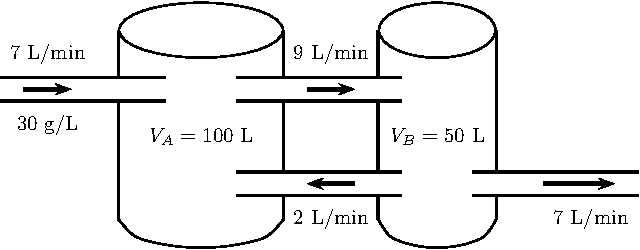
\includegraphics[width=0.5\linewidth]{graphics/notes_09_tanks2}

\newpage

\topic{Tank Model - Example 2 Part 2}
\begin{minipage}[h]{0.5\linewidth}
\vspace{0pt}
\begin{problem}
  Predict the exact salt concentrations over time by 
  solving the system of linear differential equations
  \begin{align*}
 \frac{d}{dt}    
 \begin{bmatrix} c_A \\ c_B 
     \end{bmatrix}
 =
 \begin{bmatrix}
 -0.09 & 0.02 \\
 0.18& -0.18 \\
 \end{bmatrix}
 \begin{bmatrix} c_A \\ c_B 
     \end{bmatrix}
+ 
\begin{bmatrix}
  2.1 \\ 0 
\end{bmatrix}
  \end{align*}
\end{problem}
\end{minipage} \hfill
\begin{minipage}[h]{0.45\linewidth}
\vspace{0pt}
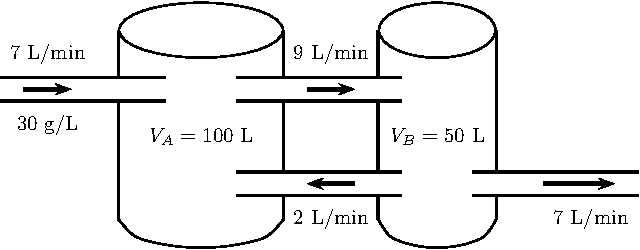
\includegraphics[width=1.0\linewidth]{graphics/notes_09_tanks2}
\end{minipage}


\newpage


~\hfill \begin{minipage}[h]{0.45\linewidth}
\vspace{0pt}
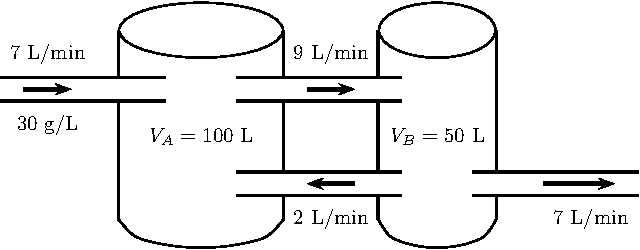
\includegraphics[width=1.0\linewidth]{graphics/notes_09_tanks2}
\LARGE
  \begin{align*}
\frac{d}{dt}    
\begin{bmatrix} c_A \\ c_B 
    \end{bmatrix}
=
\begin{bmatrix}
-0.09 & 0.02 \\
0.18& -0.18 \\
\end{bmatrix}
\begin{bmatrix} c_A \\ c_B 
    \end{bmatrix}
+ 
\begin{bmatrix}
  2.1 \\ 0 
\end{bmatrix}
  \end{align*}
\end{minipage}


\newpage

~\hfill \begin{minipage}[h]{0.45\linewidth}
\vspace{0pt}
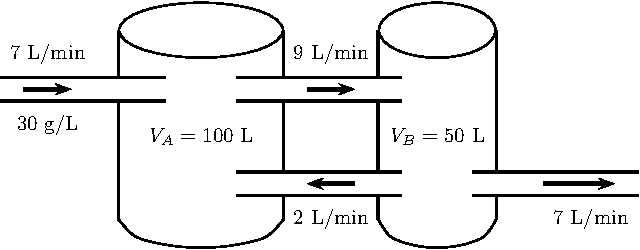
\includegraphics[width=1.0\linewidth]{graphics/notes_09_tanks2}
\LARGE
  \begin{align*}
\frac{d}{dt}    
\begin{bmatrix} c_A \\ c_B 
    \end{bmatrix}
=
\begin{bmatrix}
-0.09 & 0.02 \\
0.18& -0.18 \\
\end{bmatrix}
\begin{bmatrix} c_A \\ c_B 
    \end{bmatrix}
+ 
\begin{bmatrix}
  2.1 \\ 0 
\end{bmatrix}
  \end{align*}
\end{minipage}

\newpage
\begin{center}
  {\bf Solution} 
\end{center}
\hfill 
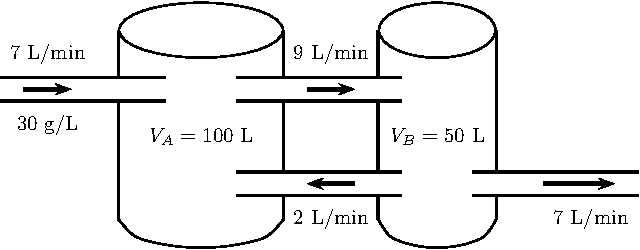
\includegraphics[width=0.4\linewidth]{graphics/notes_09_tanks2}

\begin{align*}
  c_A & = -8(2) e^{-0.06t} - 14 (1) e^{-0.21t} + 30 \\
c_B & = -8(3) e^{-0.06t} - 14 (-6)  e^{-0.21t} + 30
\end{align*}

\begin{center}
%  \includegraphics[width=0.8\linewidth]{graphics/w11_tank_graph_2}
\end{center}




\end{document}
%Confirmation of deflection:
%  http://www.efunda.com/formulae/solid_mechanics/beams/casestudy_display.cfm?case=cantilever_uniformload


\end{document}

